\section{Final evaluation}\label{sec:evaluation}

\textbf{Locked test.} Table~\ref{tab:locked} shows every model on September and October 2025, scored once. The
final model's wMAE is \usd{\TestFinalTuned} (\MapeTestFinal\% of the rate). The original CatBoost submission scores
\usd{\TestCatboostRawDollars}; its error is \usd{\TestGapCatboostRawDollars} higher (95\% interval
\TestGapCatboostRawDollarsLow{} to \TestGapCatboostRawDollarsHigh). The untuned step-5 model scores
\usd{\TestRidgePlusResidualTrees}: a difference of $\TestGapRidgePlusResidualTrees$ dollars (interval
$\TestGapRidgePlusResidualTreesLow$ to $\TestGapRidgePlusResidualTreesHigh$), slightly in its favour.

\begin{table}[H]
  \caption{Locked test, September--October 2025. ``vs final'' is the other model's clean MAE minus the final
  model's, with a 95\% paired block-bootstrap interval. Bias is the median log error.}\label{tab:locked}
  \inputtable{locked_test}
\end{table}

\textbf{Including corrupted labels.} On all rows the final model's MAE is \usd{\TestFinalAllMAE}. The difference
from the clean figure is almost entirely the corrupted labels, which no model can predict.

\textbf{Segments.} Errors are similar across equipment types and for new versus known cities, and they grow
with the forecast horizon (Table~\ref{tab:segments}).

\begin{table}[H]
  \caption{Final model on the locked test by segment (clean rows).}\label{tab:segments}
  \inputtable{segments}
\end{table}

\textbf{Residuals.} Figure~\ref{fig:residuals} shows the remaining error. From early October, actual prices sit
about \OctoberUnderForecast\% above the forecast (median, October). Daily errors are strongly autocorrelated, which means a level shift that no available
input explains.

\begin{figure}[H]
  \centering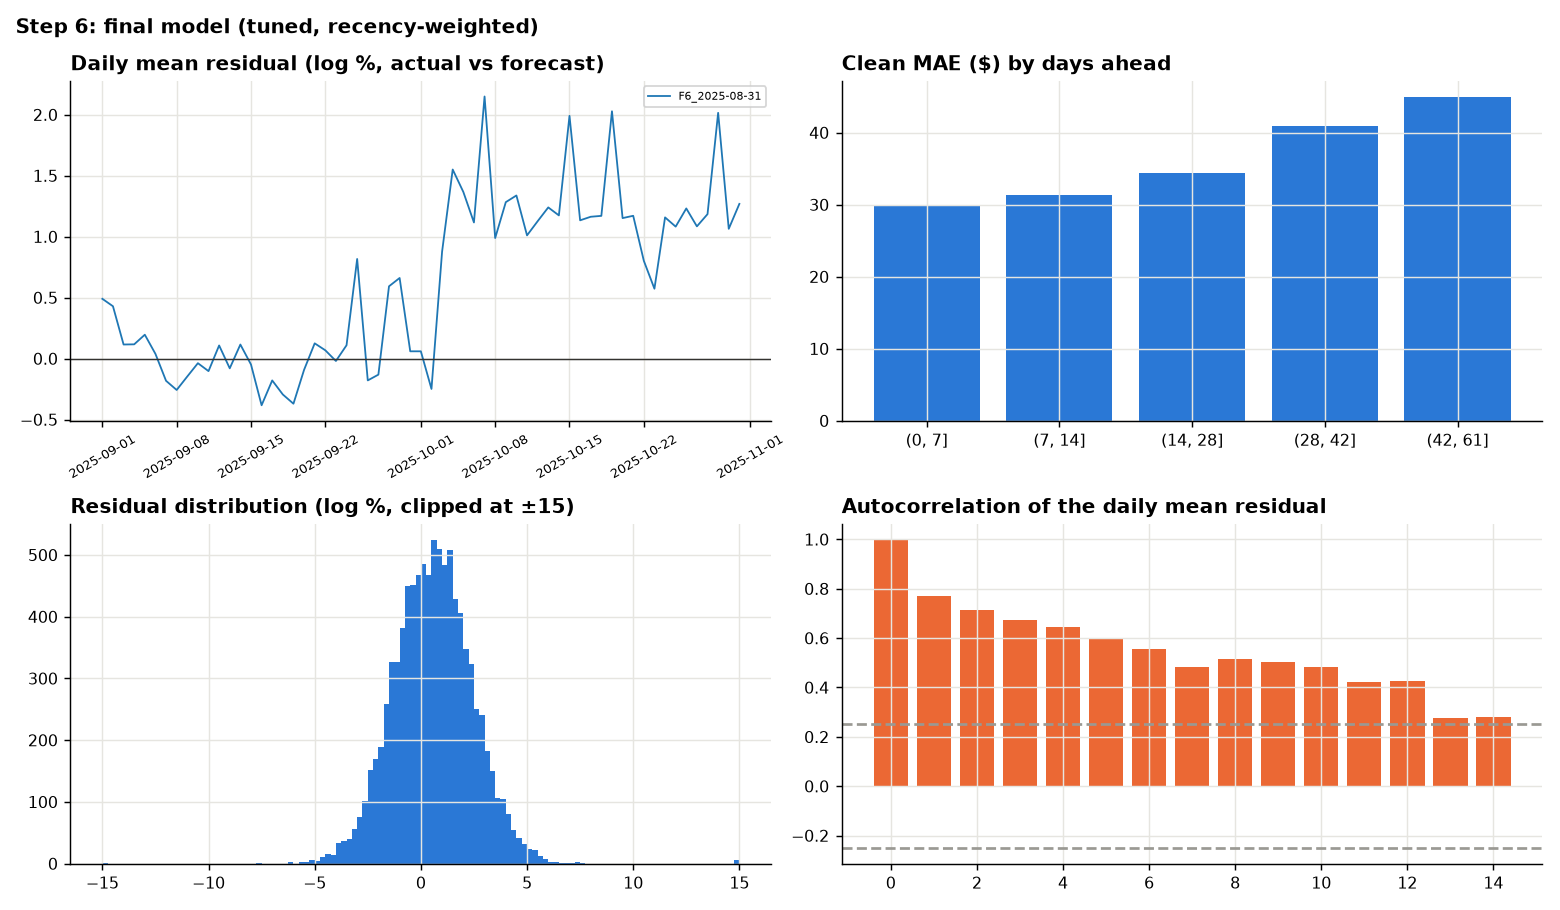
\includegraphics[width=0.95\linewidth]{residuals_test.png}
  \caption{Final model on the locked test: daily mean residual, error by horizon, residual distribution and the
  autocorrelation of daily residuals.}\label{fig:residuals}
\end{figure}

\textbf{Prediction intervals.} We take the 10th/90th and 2.5th/97.5th percentiles of the out-of-sample log errors on
the development folds, per equipment type. On the locked test the 80\% interval covers \CoverEighty\% and the 95\%
interval \CoverNinetyFive\% of clean loads (\CoverEightyAll\% and \CoverNinetyFiveAll\% of all loads). The
intervals are slightly conservative.
